%My thesis!
\documentclass[11pt,a4paper,titlepage]{report}
%\documentclass[a4paper,11pt,openright,twoside]{book}
\usepackage{amsmath}
\usepackage{ amssymb }
\usepackage{calligra}
\usepackage{amsfonts}
\usepackage[english]{babel}
\usepackage{verbatim}
\usepackage{indentfirst}
\usepackage{fancyhdr}
\usepackage{amsthm}
\usepackage{graphicx}
\usepackage{indentfirst}
\usepackage{microtype}
\usepackage{lmodern}
\usepackage{braket}
\usepackage{todonotes}

\usepackage[font=small,labelfont=bf]{caption}  %per la didascalia delle immagini
\usepackage{mathrsfs}  %per fare le lettere calligrafiche
\usepackage{bm}  %per mettere le lettere greche in grassetto
\usepackage[T1]{fontenc}     %pacchetto lettere accentate
\usepackage[utf8]{inputenc}   %pacchetto lettere accentate

\newtheorem*{remark}{Remark}

\newcommand{\HRule}{\rule{\linewidth}{0.5mm}}

% MER says: You can have no-indent later if you want to, but not while
% I'm reading this.
%\setlength\parindent{0pt} % toglie identazione ovunque
\usepackage[sc]{mathpazo}

\newcommand{\mesh}{\mathcal{T}_t}

% -----------------

\begin{document}

%--------------------------

\begin{titlepage}
%\begin{adjustwidth*}{10pt}{-40pt}
\begin{center}
\vspace*{-2.7cm}

\includegraphics{images/aquila_nome}
\\
\rule{\textwidth}{1pt}
\\[0.5cm]
{\Large DEPARTMENT OF MATHEMATICS}
\\[0.35cm]
{\Large MASTER DEGREE IN MATHEMATICS}
\\[2.3cm]
{\Large THESIS}
\\[1.5cm]
\textsc{\huge \textbf{Modeling and simulation of craniovertebral decompression}}
%\\[0.4cm]
%{\Large March 25th, 2015}
%\\[3cm]
\\[4.5cm]
\begin{minipage}{0.5\textwidth}
\flushleft {
\large Advisors: \\
 \textbf{Prof. Eleuterio F. Toro} \rule{0pt}{2.5ex}\\
 \normalsize University of Trento\\[0.4cm]
\large \textbf{Dr. Marie E. Rognes} \\
\large \textbf{Ms. Eleonora Piersanti} \\
 \normalsize Simula Research Laboratory\\[0.4cm] \rule{0pt}{2.5ex}}\\
\end{minipage}
\begin{minipage}{0.45\textwidth}
\flushright {\large
Student: \\
\rule{0pt}{2.5ex} \textbf{Carlo Cisale}\\
\normalsize University of Trento} \\
\end{minipage}

\vspace*{\fill}
{\Large ACADEMIC YEAR 2015-2016}
\rule{\textwidth}{1pt}


\end{center}
%\end{adjustwidth*}
\newpage
\thispagestyle{empty}
\phantom{}
\end{titlepage}
\newpage
\thispagestyle{empty}

%--------------------------

\tableofcontents
\pagenumbering{roman}

\newpage

\pagenumbering{arabic}

\chapter{Introduction}

\chapter{Medical background}

\chapter{Mathematical models}

\section{The Navier-Stokes equations}

\subsection{The Navier-Stokes equations on a fixed domain}

% References:
% - Quarteroni
% - Vegard
% - Drosdal

The flow in the SAS and in the spinal cord can be described by the incompressible Navier-Stokes equations for Newtonian fluids. They describe the motion of a fluid with constant density $\rho$ in a domain $\Omega \subset \mathbb{R}^d$ (where $d=2,3$). They read

\begin{align}
\rho \dot{\mathbf{u}} + \rho (\mathbf{u} \cdot \nabla)\mathbf{u} - \nabla \cdot \sigma(\mathbf{u},p) &= \mathbf{f},  && \mathbf{x} \in \Omega, \, t>0 \\
\nabla \cdot \mathbf{u} &= 0, && \mathbf{x} \in \Omega, \, t>0
\end{align}

We are going to solve the problem for the velocity field $\mathbf{u}(\mathbf{x},t)$, and the pressure field $p(\mathbf{x},t)$, where $\mathbf{x} = (x,y)$. The quantity $\sigma(\mathbf{u}, p)$, is the Cauchy stress tensor for a Newtonian fluid, given by

\[
\sigma(\mathbf{u}, p) = 2 \mu \epsilon(\mathbf{u}) - p \mathbb{I},
\]

where $\epsilon(\mathbf{u})$ is the symmetric strain rate tensor

\[
\epsilon(\mathbf{u}) = \frac{1}{2} (\nabla \mathbf{u} + (\nabla \mathbf{u})^T).
\]

The constant $\mu$ represents the fluid viscosity, while $\mathbf{f}$ denotes a forcing term per unit of mass. Substituting $\sigma$ in \eqref{} we obtain

\begin{align}
\rho \dot{\mathbf{u}} + \rho ( \mathbf{u} \cdot \nabla) \mathbf{u} - \nabla \cdot [ \nu (\nabla \mathbf{u} + (\nabla  \mathbf{u})^T)] +  \nabla p &= \mathbf{f},  \\
\nabla \cdot \mathbf{u} &= 0,
\end{align}

The term $(\mathbf{u} \cdot \nabla)\mathbf{u}$ describes the process of convective transport, while $- \nabla \cdot [ \mu (\nabla \mathbf{u} + (\nabla  \mathbf{u})^T)] $ describes the process of molecular diffusion~\cite{}.\\
Since $\mu$ is constant, from the continuity equation we obtain

\[
\nabla \cdot [ \mu (\nabla \mathbf{u} + (\nabla  \mathbf{u})^T)] = \mu [\Delta \mathbf{u} + \nabla(\nabla \cdot \mathbf{u})] = \mu \Delta \mathbf{u},
\]

hence the system can be written in the equivalent form

\begin{align}
\rho \dot{\mathbf{u}} + \rho ( \mathbf{u} \cdot \nabla) \mathbf{u} - \mu \Delta \mathbf{u} +  \nabla p &= \mathbf{f}, \\
\nabla \cdot \mathbf{u} &= 0.
\end{align}

In order for the problem to be well posed, it is necessary to assign an initial condition

\[
\mathbf{u} (\mathbf{x}, 0) = \mathbf{u}_0(\mathbf{x}) \quad \forall \mathbf{x} \in \Omega,
\]

where $\mathbf{u}_0$ is a given divergence-free vector field, together with suitable boundary conditions, such as

\[
\left\{
\begin{aligned}
& \mathbf{u}(\mathbf{x},t) = \phi (\mathbf{x}, t) & \forall \mathbf{x} \in \Gamma_D \\
& \left( \mu \frac{\partial \mathbf{u}}{\partial \mathbf{n}} - p\mathbf{n} \right) (\mathbf{x},t) = \psi(\mathbf{x},t) & \forall \mathbf{x} \in \Gamma_N
\end{aligned}
\right.
\]

where $\phi$ and $\psi$ are given vector functions, while $\Gamma_D$ and $\Gamma_N$ give a partition of the domain boundary $\partial \Omega$, that is $\Gamma_D 	\cup \Gamma_N = \partial \Omega, \mathring{\Gamma}_D \cap \mathring{\Gamma}_N = \emptyset$. Moreover, $\mathbf{n}$ is the outward unit normal vector to $\partial \Omega$. The second equation in [PUT REFERENCE TO THE PREVIOUS SYSTEM] can also be written in another form

\[
[ \nu (\nabla \mathbf{u} + \nabla \mathbf{u}^T)  - p\mathbf{n} ] = \psi(\mathbf{x}, t)  \quad \forall \mathbf{x} \in \Gamma_N.
\]

\begin{remark}
\normalfont{In our notation, if $\mathbf{u} = (u_x, u_y)^T$ and $\mathbf{x} = (x, y)^T$, then $\nabla \mathbf{u}$ is defined as

\[
\nabla \mathbf{u} =
\begin{pmatrix}
\frac{\partial u_x}{\partial x} & \frac{\partial u_x}{\partial y} \\
\frac{\partial u_y}{\partial x} & \frac{\partial u_y}{\partial y}
\end{pmatrix}
\]


}
\end{remark}

%--------------
% This is from the channel_flow.py , I don't need this

%We now want to solve N-S equations. The problem reads: find the velocity $u(x,y,t)$ and the pressure $p(x,y,t)$ such that
%
%\[
%\begin{cases}
%\rho \dot{u} + \rho (\nabla u \cdot u) - \nabla \cdot (\nu \nabla u - pI) = f, & \mbox{in } \Omega \\
%\nabla \cdot u = 0, & \mbox{in } \Omega
%\end{cases}
%\]
%
%As initial conditions (IC), we set $u(t=0) = u_0 = 0$. \\
%As boundary conditions (BC), we use
%
%\[
%\begin{cases}
%u(x,y,t) = u_{inflow}(x,y,t) , & \mbox{on } \partial \Omega_{top} \\
%u(x,y,t) = u_{outflow}(x,y,t) , & \mbox{on } \partial \Omega_{bottom} \\
%\sigma \cdot \vec{n} = 0,  & \mbox{on } \partial \Omega_{sides}
%\end{cases}
%\]
%
%where $\sigma = \nu \nabla u - pI$, and for this example
%
%\begin{equation}
%u_{inflow} = u_{outflow} =  \left[ \begin{array}{c} 0 \\ x(x-1)sin(\pi \omega x) \end{array} \right].
%\end{equation}

%--------

%\subsection{Derivation of the Navier-Stokes equations}

\subsection{Navier-Stokes on a moving domain}% -- ALE formulation}

%\subsection{The Arbitrary Lagrangian Eulerian description}

%\subsection{ALE formulation of Navier-Stokes equations}

Our next step is to allow the domain and its boundary to move, and
solve the Navier-Stokes equations on this deforming domain. Let
$\Omega_t$ denote the fluid domain which depends on time $t$. Let
$\Omega_0$ denote the fixed fluid domain at $t = 0$. In
fluid-structure interaction, the fluid domain $\Omega_t$ consists of
the same material particles at all times, and moves with the material
points within the structure. Also assume that we have a mesh $\mesh$
of the domain $\Omega_t$. Let $\mathbf{w}$ denote the \emph{mesh
  velocity}, and $\mathbf{y}$ the \emph{mesh displacement} with
respect to the reference domain $\Omega_0$, and thus by definition
$\dot{\mathbf{y}} = \mathbf{w}$ where the superposed dot denotes the
time derivative. The mesh velocity can be chosen arbitrarily in
principle, but this choice could effect the accuracy of the
solution~\cite{}.

The movement of the domain $\Omega_t$ is governed by the mesh
displacement, i.e.~for all $x(t) \in \Omega_t$, each corresponding to
a point $x_0 \in \Omega_0$, we have that
\begin{equation}
  x(t) = x_0 + \mathbf{y}(t)(x_0).
\end{equation}
\todo[inline]{Check the precise formulation carefully in Donea
  reference e.g.}

An ALE formulation of the Navier-Stokes equations on the deforming
domain $\Omega_t$ reads: find the velocity $\mathbf{u}$ and the
pressure $p$ such that
\begin{align}
  \label{eq:ns:1}
  \rho \dot{\mathbf{u}}
  + \rho [(\mathbf{u - w}) \cdot \nabla] \mathbf{u}
  - \mu \Delta \mathbf{u} + \nabla p
  &= \mathbf{f},  & \text{in } \Omega_t, \\
  \label{eq:ns:2}
  \nabla \cdot \mathbf{u} &= 0, & \text{in } \Omega_t,
\end{align}
for $t \in (0, T]$ where $\mathbf{f}$ is a given body force, $\rho$ is
  the fluid density, $\mu$ is the fluid viscosity. The
  system~\eqref{eq:ns:1}--\eqref{eq:ns:2} must be closed by
  appropriate boundary and initial conditions.

We will let the fluid domain boundary follow the changes on the
fluid-structure interface. Moreover, to move the entire domain, we
will use a \emph{Laplacian smoothing}
algorithm~\cite{Winslow1963}. More precisely, our mesh smoothing
equation reads: given a boundary velocity $\mathbf{u}_0$, find
$\mathbf{w}$ that satisfies
\begin{equation}
%\left\{
\begin{aligned}
- \Delta \mathbf{w} &= 0 	&& \text{in } \Omega_t, \\
\mathbf{w} &= \mathbf{u}_0 && \text{on } \partial \Omega_t .
\end{aligned}
%\right.
\end{equation}
for each $t \in [0, T]$


%\section{Navier-Stokes + ALE with elastic walls (Eleonora)}
%
%Starting from the previous case, we introduce a new equation to the system
%
%\[
%\left\{
%\begin{aligned}
%&\frac{\partial \mathbf{u}}{\partial t} + [(\mathbf{u - w}) \cdot \nabla] \mathbf{u} - \nu \Delta \mathbf{u} + \frac{1}{\rho} \nabla p = \frac{1}{\rho} \mathbf{f},  & x \in \Omega_t, \, t>0 \\
%& \nabla \cdot \mathbf{u} = 0, & x \in \Omega_t, \, t>0 \\
%& \mathbf{u} = (0, -2cos(4 \pi t) x(x-1) )^T, & x \in \Omega_{up} \\
%& \mathbf{u} = (0,0)^T, & x \in \Omega_{down} \\
%& \mathbf{w} = \dot{\mathbf{y}} & \text{on } \partial \Omega_t \\
%& (\sigma \cdot \hat{\mathbf{n}}) \cdot \hat{\mathbf{y}} = ky & \text{on } \partial \Omega_{spring} \\
%& \mathbf{u} = \dot{\mathbf{y}} = \frac{\partial \mathbf{y}}{\partial t}  & \text{on } \partial \Omega_{t} \\
%\end{aligned}
%\right.
%\]
%
%where $k$ is an elastic constant.

\section{Modelling the SAS with elastic surroundings}

\begin{figure}
  \caption{Left: spinal cord in the SAS. Right: Schematic illustration
    of computational domain}
\end{figure}

We will consider a fluid domain $\Omega_t$ representing a section of
the subarachnoid space between the spinal cord and the surrounding
tissue.

Assuming axial symmetry along the spinal cord length axes, we consider
a two-dimensional rectangular reference domain $\Omega_0 = [0, L_x]
\times [0, L_y]$. We define the
\begin{itemize}
\item
  top boundary: $\partial \Omega_{\rm top}^0 = \{ (x_0, x_1) | x_1 = L_y\}$;
\item
  bottom boundary: $\partial \Omega_{\rm bottom}^0 = \{ (x_0, x_1) | x_1 = 0\}$;
\item
  tissue boundary: $\partial \Omega_{\rm tissue}^0 = \{ (x_0, x_1) | x_0 = L_x\}$;
\item
  cord boundary: $\partial \Omega_{\rm cord}^0 = \{ (x_0, x_1) | x_0 = 0\}$;
\end{itemize}
and thus $\partial \Omega^0 = \partial \Omega_{\rm top}^0 \cup
\partial \Omega_{\rm bottom}^0 \cup \partial \Omega_{\rm cord}^0 \cup
\partial \Omega_{tissue}^0$. Further,
\begin{equation}
  \partial \Omega^t_{\rm i} = \partial \Omega^0_{\rm i} + \mathbf{y}(t)(\partial \Omega^0_{\rm i}),
\end{equation}
for each $i$.

We are interested in studying the effect of craniovertebral
decompression on the fluid flow and pressure dynamics in the
subarachnoid space. In particular, we assume that craniovertebral
decompression induces a change in the compliance of the tissue
surrounding the spinal canal~\cite{}. For simplicity, we aim to model
the compliance of the surrounding tissue via a boundary condition for
the fluid flow. We will assume that the tissue boundary $\partial
\Omega_{\rm tissue}$ is elastic with stiffness $k$ and in particular
allowed to move. To this end, we introduce the boundary condition
\begin{equation}
  \left ( \mu \nabla \mathbf{u} - p I
  \right ) \cdot \mathbf{n} = \pm k \mathbf{y}
  \qquad \text{ on }  \partial \Omega_{\rm tissue},
\end{equation}
where $\mathbf{n}$ is the outward pointing boundary normal and
$\mathbf{y}$ still denotes the mesh displacement. For simplicity, on
the spinal cord side, we assume that the cord is rigid and fixed,
i.e.:
\begin{equation}
  \mathbf{u} = \mathbf{0} \quad \text { on } \partial \Omega_{\rm cord}.
\end{equation}
% MER: Hmmm... This means that if y = 0, the wall is free to move.

To induce a fluid flow in the subarachnoid space, we prescribe an
inlet velocity $\tilde{u}$ on the top boundary, while on the bottom
boundary we assume that $ \left ( \mu \nabla \mathbf{u} - p I \right )
\cdot \mathbf{n} = 0$.

For the mesh equation, we let the mesh velocity follow the fluid
velocity on the tissue boundary, while the mesh velocity is assumed to
be zero (i.e.~the mesh boundary is fixed) on the remaining boundary:
\begin{align}
\mathbf{w} &= \mathbf{u}  \qquad \text{ on } \partial \Omega_{\rm tissue},\\
\mathbf{w} &= \mathbf{0}  \qquad \text{ on } \partial \Omega^t \setminus \partial \Omega_{\rm tissue}
\end{align}

Note that $\partial \Omega_{\rm cord}$ and $\partial \Omega_{\rm
  tissue}$ are \textit{physical} boundaries, i.e.~they model portions
of the spinal cord and surrounding tissue. This means that
$\mathbf{u}$ and $\mathbf{w}$ should have the same value on these
boundaries, since the fluid follows the movement (if any) of the
walls.

\section{Navier-Stokes + ALE with elastic walls (Marie)}
Let us start with Navier-Stokes encountering the ALE term. The problem reads:

\[
\begin{aligned}
\rho \frac{\partial u}{\partial t} + \rho \nabla u \cdot (u-w) - div(\nu \nabla u) + \nabla p = f  , & \text{ in } \Omega_F (t), \\
div u = 0, & \text{ in } \Omega_F (t), \\
\end{aligned}
\]

for give $\rho, \nu, f$ and mesh velocity $w$.

As boundary conditions on the fluid domain we choose

\[
\begin{aligned}
u = w, & \text{ on } \partial \Omega_C \cup \partial \Omega_T \\
(\nu \nabla u - pI) \cdot n = p_0 n, & \text{ on } \partial \Omega_{TB}
\end{aligned}
\]

We define the mesh velocity as $w = \dot{y}$, where $y$ is the mesh displacement. \\
Smoothing of the mesh:

\[
\begin{aligned}
- \Delta y = 0, & \text{ on } \partial \Omega_F (t), \\
y = 0, & \text{ on } \partial \Omega_{TB}, \\
\end{aligned}
\]

where the condition $y = 0$ is equivalent to no movement on the top and bottom of the boundary. \\
We consider two different models:

\begin{description}
\item[option 1:] we allow the movement of the boundary in every direction by imposing the condition

\[
- \nabla y \cdot n = (\pm)ky \qquad \text{ on } \partial \Omega_C \cup \partial \Omega_T \\
\]

where $k = k(x)$ is the spring constant;

\item[option 2:] we allow the movement of the boundary only in the normal direction, that means

\[
\begin{aligned}
(- \nabla y \cdot n) \cdot n = (\pm)ky \cdot n & \qquad \text{normal direction} \\
y \cdot t = 0 & \qquad \text{tangential direction}
\end{aligned}
\]

where $n$ is the normal vector to the boundary, and $t$ is the tangent to the boundary. \\
This can be done "weakly" using the Nitsche's method (check André Massing PhD thesis).

\end{description}

We are going to consider 3 different steps (or models):

\begin{description}
\item[Model 1:] we suppose

\[
\begin{aligned}
y = 0 & \qquad \text{ on } \partial \Omega_{TB}, \partial \Omega_C \\
k = fixed & \qquad \text{ on } \partial \Omega_{T (tissue)}
\end{aligned}
\]

\item[Model 2:] as model 1, but $k$ varies with $x_1$
\item[Model 3-4:] as model 1-2, but letting also $\partial \Omega_C$ have a $k$ (so the cord is elastic).

\end{description}





\chapter{Numerical methods}

\section{Finite element formulation}

\subsection{Weak formulation of Stokes equations}

\todo[inline]{Do I need to keep this subsection?}

In order to find a numerical solution to this problem, we write its variational formulation. Let $\mathbf{v}$ be a test function in the space $\hat{V} = \set{\mathbf{u} \in H^1(\Omega) | \mathbf{u}_{|_{\partial \Omega}} = 0} $. Our aim is to find $(\mathbf{u}(x,y),p(x,y)) \in V \times Q$ such that

\begin{align}
\int_\Omega -\nabla \cdot (\nu \nabla \mathbf{u} - pI)\mathbf{v} \,dx &= \int_\Omega f \mathbf{v} \,dx, \\
\int_\Omega (\nabla \cdot \mathbf{u})q \,dx &= 0
\end{align}

Differentiating by part the right hand side of the first equation we obtain:

\begin{align}
\int_\Omega -\nabla \cdot (\nu \nabla \mathbf{u} - pI)\mathbf{v} \,dx &= \int_\Omega (\nu \nabla \mathbf{u} - pI) \cdot \nabla \mathbf{v} \,dx, \\
&- \int_{\partial \Omega} (\nu \nabla \mathbf{u} - pI) \cdot n \mathbf{v} \,ds.
\end{align}

Since we set Dirichlet boundary conditions on the entire boundary and $\mathbf{v}_{|_{\partial \Omega}} = 0$, the boundary integral is zero. Hence, our weak formulation reads

\begin{align}
\int_\Omega (\nu \nabla \mathbf{u} - pI) \cdot \nabla \mathbf{v} \,dx &= \int_\Omega f\mathbf{v} \,dx, \\
\int_\Omega (\nabla \cdot \mathbf{u}) q \,dx &= 0.
\end{align}

Instead of using the space $V \times Q$, we use $V_h \times Q_h$, where $V_h$ and $Q_h$ are spaces defined with respect to a mesh $J_h$. We hence seek $(u_h, p_h) \in V_h \times Q_h$, where $V_h = \mathcal{P}^{cont,d}_{k+1} (J_h)$ and $Q_h = \mathcal{P}^{cont}_{k} (J_h)$ (typically we choose $k=1$). \\


Since the pressure is defined up to some constant, we add the constraint

\[
\frac{1}{|\Omega |} \int_{\Omega} p = 0,
\]

so we can compare an exact solution with mean value zero with the approximate solution.

\subsection{Weak formulation of Navier-Stokes equations}


In order to solve this problem numerically using finite element method, we write its variational form. Let $v$ be a test function in

\[
\hat{V} = \set{\mathbf{v} \in H^1(\Omega) | v_{|_{\partial \Omega_{top} \, \cup \, \partial \Omega_{bottom}}} = 0}
\]

and $q \in \hat{Q}$. Let us multiply the N-S equations by $\mathbf{v}$ and $q$ and integrate on $\Omega$:

\begin{align}
&\int_{\Omega} \rho \, \dot{\mathbf{u}} \, \mathbf{v} \, dx
+ \int_{\Omega} \rho (\nabla \mathbf{u} \cdot \mathbf{u} )\mathbf{v} \, dx
- \int_{\Omega} \nabla \cdot (\mu \nabla \mathbf{u} - pI)\mathbf{v} \, dx
= \int_{\Omega} f\mathbf{v} \, dx \\
&\int_{\Omega} (\nabla \cdot \mathbf{u}) q \, dx = 0.
\end{align}

I take the term $- \int_{\Omega} \nabla \cdot (\mu \nabla \mathbf{u} - pI)\mathbf{v} \, dx$, and integrate by parts:

\[
- \int_{\Omega} \nabla \cdot (\mu \nabla \mathbf{u} - pI)\mathbf{v} \, dx
= \int_{\Omega} (\mu \nabla \mathbf{u} - pI) \cdot \nabla \mathbf{v} \, dx
- \int_{\partial \Omega} (\mu \nabla \mathbf{u} - pI) \cdot \mathbf{n} \, \mathbf{v} \, dx.
\]

The boundary term can actually be divided in three different terms (one for each part of the boundary), as $\partial \Omega = \partial \Omega_{top} \cup \partial \Omega_{bottom} \cup \partial \Omega_{sides}$. Since we chose $\mathbf{v} \in \hat{V}$, the term on $\partial \Omega_{top} \cup \partial \Omega_{bottom}$ is zero. The term on $\partial \Omega_{sides}$ is also zero: since $\sigma = \mu \nabla \mathbf{u} - pI$ and $\sigma \cdot \mathbf{n} = 0$ on $\partial \Omega_{sides}$, the remaining term on the boundary is also zero. Hence, $- \int_{\partial \Omega} (\mu \nabla \mathbf{u} - pI) \cdot \mathbf{n} \, \mathbf{v} \, dx = 0$.

The variational form becomes

\begin{align}
\int_{\Omega} \rho \, \dot{\mathbf{u}} \, \mathbf{v} \, dx
+ \int_{\Omega} \rho (\nabla \mathbf{u} \cdot \mathbf{u})\mathbf{v} \, dx
- \int_{\Omega} (\mu \nabla \mathbf{u} - pI) \cdot \nabla \mathbf{v} \, dx
&= \int_{\Omega} f\mathbf{v} \, dx \\
\int_{\Omega} (\nabla \cdot \mathbf{u}) q \, dx &= 0.
\end{align}


\subsection{Weak formulation of Navier-Stokes and ALE}

% variational form for N-S
% variational form for Poisson problem for w

From [PUT REFERENCE TO EQUATION WITH w], we multiply by a test function $v$ the first equation and by the test function $q$ the second equation, and integrate over $\Omega$. We hence obtain:

\begin{align*}
\int_{\Omega} \rho \dot{\mathbf{u}} \, \mathbf{v} \, dx
+ \int_{\Omega} \rho [(\mathbf{u - w}) \cdot \nabla] \mathbf{u} \, \mathbf{v} \, dx
- \int_{\Omega} \nabla \cdot (\mu \nabla \mathbf{u} -  pI)\mathbf{v} \, dx
&=  \int_{\Omega} \mathbf{f} \, dx, \\
 \int_{\Omega}  (\nabla \cdot \mathbf{u}) q \, dx &= 0.
\end{align*}

As before, the term $- \int_{\Omega} \nabla \cdot (\mu \nabla \mathbf{u} - pI)\mathbf{v} \, dx$ can be integrated by parts:

\[
- \int_{\Omega} \nabla \cdot (\mu \nabla \mathbf{u} - pI)\mathbf{v} \, dx
=  \int_{\Omega} (\mu \nabla \mathbf{u} - pI) \cdot \nabla \mathbf{v} \, dx
- \int_{\partial \Omega} (\mu \nabla \mathbf{u} - pI) \cdot \mathbf{n} \, \mathbf{v} \, ds.
\]

The boundary $\partial \Omega$ can be divided in two boundaries $ \partial \Omega = \partial \Omega_D \cup \partial \Omega_N $, where $\partial \Omega_D$ and $\partial \Omega_N$ are respectively the Dirichlet boundary and the Neumann boundary.
Since we chose $\mathbf{v} \in \hat{V}$, the term on $\partial \Omega_{D}$ is zero. The term on $\partial \Omega_{D}$ is also zero: since $\sigma = \mu \nabla \mathbf{u} - pI$ and $\sigma \cdot \vec{\mathbf{n}} = 0$ on $\partial \Omega_{D}$, the remaining term on the boundary is also zero. Hence,

\[- \int_{\partial \Omega} (\mu \nabla \mathbf{u} - pI) \cdot \mathbf{n} \, \mathbf{v} \, dx = 0.\]

The variational formulation reads:

\begin{align*}
\int_{\Omega} \rho \dot{\mathbf{u}} \, \mathbf{v} \, dx
+ \int_{\Omega} \rho [(\mathbf{u - w}) \cdot \nabla] \mathbf{u} \, \mathbf{v} \, dx
+ \int_{\Omega} (\mu \nabla \mathbf{u} - pI) \cdot \nabla \mathbf{v} \, dx
&=  \int_{\Omega} \mathbf{f} \, dx,  \\
\int_{\Omega} ( \nabla \cdot \mathbf{u} ) q \, dx &= 0.
\end{align*}

We now want to write the variational formulation for the Poisson problem: let $\mathbf{z}$ be a test function in [SPECIFY THE SPACE]. Integrating by parts equation [PUT REFERENCE], we obtain

\[
\int_{\Omega} \nabla^2 \mathbf{w} \, \mathbf{z} \, dx = - \int_{\Omega} \nabla \mathbf{w} \cdot \nabla \mathbf{z} \, dx + \int_{\partial \Omega} \frac{\partial \mathbf{w}}{\partial \mathbf{n}} \mathbf{z} \, ds.
\]

Since we are assuming Dirichlet boundary conditions on the entire boundary, we choose $\mathbf{z = 0}$ everywhere, hence the term $\int_{\partial \Omega} \frac{\partial \mathbf{w}}{\partial \mathbf{n}} \, \mathbf{z} \, dx  = 0 $. Typically, the boundary $\partial \Omega_t$ will be divided into a physical and a fictitious boundary. We note as well that on the physical boundary, the values of $\mathbf{w}$ and $\mathbf{u}$ should be the same.
Finally, we obtain

\[
\int_{\Omega} \nabla^2 \mathbf{w} \, \mathbf{z} \, dx = - \int_{\Omega} \nabla \mathbf{w} \cdot \nabla \mathbf{z} \, dx = 0.
\]

The problem reads: find $\mathbf{w} \in$ [SOME SPACE TO SPECIFY] such that

\[
\begin{aligned}
-  \int_{\Omega_t} \nabla \mathbf{w} & \cdot \nabla \mathbf{z} \, dx = 0, & \text{in } \Omega_t, \\
& \mathbf{w} = \mathbf{u}, & \text{on } \partial \Omega_t
\end{aligned}
\]

$\forall \mathbf{z} \in $ [SPECIFY SPACE].

\textbf{Reminder:} in our case, we choose

\[
\begin{aligned}
\mathbf{w = u} \, & \text{ on } \partial \Omega_{Tissue}, \\
\mathbf{w = 0} \, & \text{ on } \partial \Omega_t \setminus \partial \Omega_{Tissue}.
\end{aligned}
\]

so we are allowing just the part of the boundary $\partial \Omega_{Tissue}$ to move.


\subsection{Nitsche's method}
Nitsche's method was proposed as a way for treating boundary conditions in finite element method. In particular, it is used to weakly impose boundary and interface conditions, and it is applicable to a wide class of problems. Let us use Poisson's equation as a model problem. Given a domain $\Omega$ with boundary $\Gamma = \partial \Omega$, the problem is to find $\mathbf{u}$ such that

\begin{equation}
- \Delta \mathbf{u} = \mathbf{f} \qquad \text{ in } \Omega,
\label{eq:nitsche:1}
\end{equation}

subject to the boundary condition

\begin{equation}
\mathbf{u} = \mathbf{g} \qquad \text{ on } \Gamma.
\label{eq:nitsche:2}
\end{equation}

Generally, Dirichlet boundary conditions as~\eqref{eq:nitsche:2} are strongly imposed by seeking the solution $\mathbf{u}$ in some function space $V_g$, consisting of functions that already satisfy ~\eqref{eq:nitsche:2}. The idea of Nitsche's method~\cite{Nitsche1977} is to introduce a function space $V$ that does not satisfy that requirement, while 'weakly' enforcing the boundary condition. In order to derive the weak formulation, let us multiply equation~\eqref{eq:nitsche:1} by a test function $\mathbf{v}$ and integrate by parts. We obtain 

\begin{equation}
\label{eq:nitsche:3}
\int_{\Omega} \nabla \mathbf{u} \cdot \nabla \mathbf{v} \, dx
- \int_{\Gamma} \frac{\partial \mathbf{u}}{\partial \mathbf{n}} \, \mathbf{v} \, ds
= \int_{\Omega} \mathbf{f} \mathbf{v} \, dx. 
\end{equation}

We now want to enforce the boundary condition~\eqref{eq:nitsche:2} by adding a new term 

\begin{equation}
\int_{\Omega} \nabla \mathbf{u} \cdot \nabla \mathbf{v} \, dx
- \int_{\Gamma} \frac{\partial \mathbf{u}}{\partial \mathbf{n}} \, \mathbf{v} \, dx 
+ \gamma \int_{\Gamma} \mu (\mathbf{u} - \mathbf{g}) \mathbf{v} \, ds
= \int_{\Omega} \mathbf{f} \mathbf{v} \, dx,
\end{equation}

where $\gamma > 0$ is a penalty parameter and $\mu$ is a weight to adjust the penalty of the jump. Nitsche in ~\cite{Nitsche1977} proved that the choice $\mu = \gamma h^{-1}$, with $h$ being the local mesh size, gives an optimally convergent method. In order to make the variational form symmetric, we can add the term $\int_{\Gamma} \nabla \mathbf{u} \cdot \mathbf{n} (\mathbf{u}-\mathbf{g}) \, ds$ to recover symmetry. Hence, the final Nitsche method reads:

\begin{align}
\int_{\Omega} \nabla \mathbf{u} \cdot \nabla \mathbf{v} \, dx
- \int_{\Gamma} \frac{\partial \mathbf{u}}{\partial \mathbf{n}} \, \mathbf{v} \, ds
& - \int_{\Gamma} \frac{\partial \mathbf{v}}{\partial \mathbf{n}}\, \mathbf{u} \, ds 
+ \gamma \int_{\Gamma} h^{-1} \mathbf{u} \mathbf{v} \, ds = \\
	\int_{\Omega} \mathbf{f} \mathbf{v} \, dx
&- \int_{\Gamma} \frac{\partial \mathbf{u}}{\partial \mathbf{n}} \, \mathbf{g} \, ds
+ \gamma \int_{\Gamma} h^{-1} \mathbf{g} \mathbf{v} \, ds.
\end{align}

What we would like to do now is using the previous method to weakly set boundary conditions on the normal and the tangential components of the velocity field $\mathbf{u}$. The problem is to find $\mathbf{u}$ such that
\begin{align}
- \Delta \mathbf{u} &= \mathbf{f} \quad \text{ in } \Omega, \\
\label{eq:nitsche:4}
\frac{\partial \mathbf{u}^n}{\partial \mathbf{n}} &= \mathbf{l} \quad \text{ on } \Gamma, \\ 
\mathbf{u}^t &= \mathbf{g} \quad \text{ on } \Gamma.
\end{align}

where $\mathbf{u}^n$ and $\mathbf{u}^t$ are respectively the normal and tangential components of the velocity $\mathbf{u}$, and $\mathbf{u} = \mathbf{u}^n + \mathbf{u}^t$. We then multiply by a test function $\mathbf{v}$, and substitute $\mathbf{u} = \mathbf{u}^n + \mathbf{u}^t$ and $\mathbf{v} = \mathbf{v}^n + \mathbf{v}^t$ in~\eqref{eq:nitsche:3}, obtaining

\begin{equation}
\int_\Omega \nabla \mathbf{u} \cdot \nabla \mathbf{v} dx
- \int_{\Gamma} \frac{\partial \mathbf{u}^n}{\partial \mathbf{n}} \mathbf{v}^n \, ds
- \int_{\Gamma} \frac{\partial \mathbf{u}^t}{\partial \mathbf{n}} \mathbf{v}^t \, ds
= \int_\Omega \mathbf{fv} \, dx.
\end{equation}

From the boundary condition~\eqref{eq:nitsche:4}, I obtain

\begin{equation}
\int_\Omega \nabla \mathbf{u} \cdot \nabla \mathbf{v} dx
- \int_{\Gamma} \frac{\partial \mathbf{u}^t}{\partial \mathbf{n}} \mathbf{v}^t \, ds
=  \int_{\Gamma} \mathbf{l} \mathbf{v}^n \, ds
+ \int_\Omega \mathbf{fv} \, dx
\end{equation}

Applying the Nitsche method on the boundary term in the left hand side, we get

\begin{align}
\int_\Omega \nabla \mathbf{u} \cdot \nabla \mathbf{v} dx
- \int_{\Gamma} \frac{\partial \mathbf{u}^t}{\partial \mathbf{n}} \mathbf{v}^t \, ds
- \int_{\Gamma} \frac{\partial \mathbf{v}^t}{\partial \mathbf{n}} \mathbf{u}^t \, ds
&+ \gamma \int_{\Gamma} h^{-1} \mathbf{u}^t \mathbf{v}^t \, ds = \\
	 \int_{\Gamma} \mathbf{l} \mathbf{v}^n \, ds
+ \int_\Omega \mathbf{fv} \, dx
 - \int_{\Gamma} \frac{\partial \mathbf{v}^t}{\partial \mathbf{n}} \mathbf{g} \, ds
&+ \gamma \int_{\Gamma} h^{-1} \mathbf{g} \mathbf{v}^t \, ds
\end{align}

\subsection{Weak formulation of  ALE + elastic (Eleonora)}
From [PUT REFERENCE TO EQUATION WITH w], we multiply by a test function $\mathbf{v}$ the first equation and by the test function $q$ the second equation, and integrate over $\Omega$. We obtain:
\begin{align*}
\int_{\Omega} \rho \dot{\mathbf{u}} \, \mathbf{v} \, dx
+ \int_{\Omega} \rho [(\mathbf{u - w}) \cdot \nabla] \mathbf{u} \, \mathbf{v} \, dx
- \int_{\Omega} \nabla \cdot (\mu \nabla \mathbf{u} - pI)\mathbf{v} \, dx
&= \int_{\Omega} \mathbf{f} \mathbf{v} \, dx, \\
\int_{\Omega}  (\nabla \cdot \mathbf{u}) q \, dx &= 0.
\end{align*}

As before, the term $- \int_{\Omega} \nabla \cdot (\mu \nabla \mathbf{u} - pI)\mathbf{v} \, dx$ can be integrated by parts:

\[
- \int_{\Omega} \nabla \cdot (\mu \nabla \mathbf{u} - pI)\mathbf{v} \, dx =  \int_{\Omega} (\mu \nabla \mathbf{u} - pI) \cdot \nabla \mathbf{v} \, dx - \int_{\partial \Omega} (\mu \nabla \mathbf{u} - pI) \cdot \mathbf{n} \, \mathbf{v} \, ds.
\]

The boundary $\partial \Omega_t$ can be divided in the four boundaries:

\[
\partial \Omega_t= \partial \Omega_{Top} \cup \partial \Omega_{Bottom} \cup \partial \Omega_{Cord} \cup  \partial \Omega_{Tissue}.
\]

On $\partial \Omega_{Top}$ and $\partial \Omega_{Cord}$ we assume Dirichlet boundary conditions for the velocity $\mathbf{u}$, hence the test function $\mathbf{v}$ will be zero on these two boundaries. Moreover, I assumed $\sigma \cdot \mathbf{n} = 0$ on $\partial \Omega_{Bottom}$, while $\sigma \cdot \mathbf{n} = \pm k \mathbf{y} $ on $\partial \Omega_{Tissue}$, where $\mathbf{y}$ is the mesh displacement vector. The boundary term becomes

\[
- \int_{\partial \Omega_t} (\mu \nabla \mathbf{u} - p I) \cdot \, \mathbf{n} \, \mathbf{v} \, dx = - \int_{\partial \Omega_{Tissue}} (\pm k \mathbf{y}) \, \mathbf{v} \, dx.
\]

The variational formulation reads:

\begin{align*}
\int_{\Omega} \rho \dot{\mathbf{u}} \, \mathbf{v} \, dx
+ \int_{\Omega} \rho [(\mathbf{u - w}) \cdot \nabla] \mathbf{u} \, \mathbf{v} \, dx
+ \int_{\Omega} (\nu \nabla \mathbf{u} - pI) \cdot \nabla \mathbf{v} \, dx \\
- \int_{\partial \Omega_{tissue}} (\pm k \mathbf{y}) \, \mathbf{v} \, dx
=  \int_{\Omega} \mathbf{f} \mathbf{v} \, dx.
\end{align*}

We now would like to set the tangential component of the velocity to $0$, in order to allow the mesh to move just in the normal direction of the $\partial \Omega_{tissue}$ boundary.

\todo[inline]{We also need another condition for the normal direction, WHICH ONE? TO WRITE PRECISELY}

We start from 

\[
 \int_{\Omega} \rho \dot{\mathbf{u}} \, \mathbf{v} \, dx
+ \int_{\Omega} \rho [(\mathbf{u - w}) \cdot \nabla] \mathbf{u} \, \mathbf{v} \, dx
- \int_{\Omega} \nabla \cdot (\mu \nabla \mathbf{u} - pI)\mathbf{v} \, dx
= \int_{\Omega} \mathbf{f} \mathbf{v} \, dx
\]

I integrate by parts and obtain 

\begin{align*}
 \int_{\Omega} \rho \dot{\mathbf{u}} \, \mathbf{v} \, dx
+ \int_{\Omega} \rho [(\mathbf{u - w}) \cdot \nabla] \mathbf{u} \, \mathbf{v} \, dx
+ \int_{\Omega} (\mu \nabla \mathbf{u} - pI) \cdot \nabla \mathbf{v} \, dx \\
- \int_{\partial \Omega} (\mu \nabla \mathbf{u} - pI) \cdot \mathbf{n} \, \mathbf{v} \, ds
= \int_{\Omega} \mathbf{f} \mathbf{v} \, dx
\end{align*}

According to the boundary conditions, the boundary term $\partial \Omega_{tissue}$ is the only one that survives, hence

\begin{align*}
 \int_{\Omega} \rho \dot{\mathbf{u}} \, \mathbf{v} \, dx
+ \int_{\Omega} \rho [(\mathbf{u - w}) \cdot \nabla] \mathbf{u} \, \mathbf{v} \, dx
+ \int_{\Omega} (\mu \nabla \mathbf{u} - pI) \cdot \nabla \mathbf{v} \, dx \\
- \int_{\partial \Omega_{tissue}} (\mu \nabla \mathbf{u} - pI) \cdot \mathbf{n} \, \mathbf{v} \, ds
= \int_{\Omega} \mathbf{f} \mathbf{v} \, dx
\end{align*}

Since $\nabla \mathbf{u} \cdot \mathbf{n} = \frac{\partial \mathbf{u}}{\partial \mathbf{n}}$, I can rewrite the boundary term:

\[
\int_{\partial \Omega_{tissue}} (\mu \nabla \mathbf{u} -  pI) \cdot \mathbf{n} \, \mathbf{v} \, ds = \int_{\partial \Omega_{tissue}} (\mu \frac{\partial \mathbf{u}}{\partial \mathbf{n}} -  p \mathbf{n}) \, \mathbf{v} \, ds.
\]


We can see the vector field $\mathbf{u}$ as the sum of its normal and tangential components, i.e. $\mathbf{u} = \mathbf{u}^n + \mathbf{u}^t$. The same can be said for the test function $\mathbf{v} = \mathbf{v}^n + \mathbf{v}^t$. We then substitute $\mathbf{u}$ and $\mathbf{v}$ in the boundary term:

\begin{align*}
& \int_{\partial \Omega_{tissue}} (\mu \frac{\partial \mathbf{u}}{\partial \mathbf{n}} -  p \mathbf{n}) \, \mathbf{v} \, ds = \\
& \int_{\partial \Omega_{tissue}} (\mu \frac{\partial (\mathbf{u}^n + \mathbf{u}^t)}{\partial \mathbf{n}} -  p \mathbf{n}) \, \mathbf{v} \, ds = \\
& \int_{\partial \Omega_{tissue}} (\mu \frac{\partial (\mathbf{u}^n + \mathbf{u}^t)  }{\partial \mathbf{n}} \mathbf{v} \,ds - \int_{\partial \Omega_{tissue}} p \mathbf{n} \, \mathbf{v} \, ds = \\
& \int_{\partial \Omega_{tissue}} \mu \frac{\partial \mathbf{u}^t}{\partial \mathbf{n}} \mathbf{v} \, ds
+ \int_{\partial \Omega_{tissue}} \mu \frac{\partial \mathbf{u}^n}{\partial \mathbf{n}} \mathbf{v} \, ds
- \int_{\partial \Omega_{tissue}} p \mathbf{n} \, \mathbf{v} \, ds = \\
& \int_{\partial \Omega_{tissue}} \mu \frac{\partial \mathbf{u}^t}{\partial \mathbf{n}} \mathbf{v} \, ds 
+ \int_{\partial \Omega_{tissue}} ( \mu \frac{\partial \mathbf{u}^n}{\partial \mathbf{n}} - p \mathbf{n} ) \mathbf{v} \, ds = \\
& \int_{\partial \Omega_{tissue}} \mu \frac{\partial \mathbf{u}^t}{\partial \mathbf{n}} (\mathbf{v}^n + \mathbf{v}^t) \, ds 
+ \int_{\partial \Omega_{tissue}} ( \mu \frac{\partial \mathbf{u}^n}{\partial \mathbf{n}} - p \mathbf{n} ) \mathbf{v} \, ds = \\
& \int_{\partial \Omega_{tissue}} \mu \frac{\partial \mathbf{u}^t}{\partial \mathbf{n}} \mathbf{v}^t \, ds 
+ \int_{\partial \Omega_{tissue}} ( \mu \frac{\partial \mathbf{u}^n}{\partial \mathbf{n}} - p \mathbf{n} ) \mathbf{v} \, ds. \\
\end{align*}

\todo[inline]{where the last equality is due to the fact that the spaces are in direct sum? Tangential component multiplied by normal derivative is 0, VERIFY}

The variational form of Navier-Stokes becomes

\begin{align*}
 \int_{\Omega} \rho \dot{\mathbf{u}} \, \mathbf{v} \, dx
+ \int_{\Omega} \rho [(\mathbf{u - w}) \cdot \nabla] \mathbf{u} \, \mathbf{v} \, dx
+ \int_{\Omega} (\mu \nabla \mathbf{u} - pI) \cdot \nabla \mathbf{v} \, dx \\
- \int_{\partial \Omega_{tissue}} \mu \frac{\partial \mathbf{u}^t}{\partial \mathbf{n}} \mathbf{v}^t \, ds 
- \int_{\partial \Omega_{tissue}} ( \mu \frac{\partial \mathbf{u}^n}{\partial \mathbf{n}} - p \mathbf{n} ) \mathbf{v} \, ds
= \int_{\Omega} \mathbf{f} \mathbf{v} \, dx
\end{align*}

then I apply the Nitsche method on the first boundary term: 

\begin{align*}
& \int_{\Omega} \rho \dot{\mathbf{u}} \, \mathbf{v} \, dx
+ \int_{\Omega} \rho [(\mathbf{u - w}) \cdot \nabla] \mathbf{u} \, \mathbf{v} \, dx
+ \int_{\Omega} (\mu \nabla \mathbf{u} - pI) \cdot \nabla \mathbf{v} \, dx \\
& - \int_{\partial \Omega_{tissue}} \mu \frac{\partial \mathbf{u}^t}{\partial \mathbf{n}} \mathbf{v}^t \, ds 
- \int_{\partial \Omega_{tissue}} \mu \frac{\partial \mathbf{v}^t}{\partial \mathbf{n}} \mathbf{u}^t \, ds 
+ \int_{\partial \Omega_{tissure}} \frac{\gamma}{h} \mathbf{u}^t \mathbf{v}^t \, ds \\
& - \int_{\partial \Omega_{tissue}} ( \mu \frac{\partial \mathbf{u}^n}{\partial \mathbf{n}} - p \mathbf{n} ) \mathbf{v} \, ds \\
& =  \int_{\Omega} \mathbf{f} \mathbf{v} \, dx
- \int_{\partial \Omega_{tissue}} \mu \frac{\partial \mathbf{v}^t}{\partial \mathbf{n}} \mathbf{g} \, ds 
+ \int_{\partial \Omega_{tissure}} \frac{\gamma}{h} \mathbf{g} \mathbf{v}^t \, ds
\end{align*}

\todo[inline]{My problem is: what about the second term? I should substitute it with the term $k \mathbf{y}$, but what is the right condition that we use?}

Then I substitute:

\[
- \int_{\partial \Omega_{tissue}} ( \mu \frac{\partial \mathbf{u}^n}{\partial \mathbf{n}} - p \mathbf{n} ) \mathbf{v} \, ds
= - \int_{\partial \Omega_{tissue}} (k \mathbf{y}) \cdot \mathbf{n} ds 
\]

where $k < 0$ (that term should be positive otherwise I have problems). Hence

\begin{align*}
& \int_{\Omega} \rho \dot{\mathbf{u}} \, \mathbf{v} \, dx
+ \int_{\Omega} \rho [(\mathbf{u - w}) \cdot \nabla] \mathbf{u} \, \mathbf{v} \, dx
+ \int_{\Omega} (\mu \nabla \mathbf{u} - pI) \cdot \nabla \mathbf{v} \, dx \\
& - \int_{\partial \Omega_{tissue}} \mu \frac{\partial \mathbf{u}^t}{\partial \mathbf{n}} \mathbf{v}^t \, ds 
- \int_{\partial \Omega_{tissue}} \mu \frac{\partial \mathbf{v}^t}{\partial \mathbf{n}} \mathbf{u}^t \, ds 
+ \int_{\partial \Omega_{tissure}} \frac{\gamma}{h} \mathbf{u}^t \mathbf{v}^t \, ds \\
& - \int_{\partial \Omega_{tissue}} (k \mathbf{y}) \cdot \mathbf{n} ds  \\
& = \int_{\Omega} \mathbf{f} \mathbf{v} \, dx
- \int_{\partial \Omega_{tissue}} \mu \frac{\partial \mathbf{v}^t}{\partial \mathbf{n}} \mathbf{g} \, ds 
+ \int_{\partial \Omega_{tissure}} \frac{\gamma}{h} \mathbf{g} \mathbf{v}^t \, ds
\end{align*}

%\subsection{Weak Formulation of ALE + elastic (Marie)}
%Weak formulation for the Poisson problem
%
%\[
%\left\{
%\begin{aligned}
%-\Delta y = 0, \quad in \Omega_F (t), \\
%y = y_0,  \quad on \partial \Omega_0 (t) \\
%- \nabla y \cdot n = \pm ky \quad on \partial \Omega_1 (t)
%\end{aligned}
%\right.
%\]
%
%Weak formulation: find $y \in H^1_{y_0, \partial \Omega_0}$ such that
%
%\[
%\int_\Omega -\Delta y \cdot z = 0 \qquad \forall z \in H^1_{0, \partial \Omega_0}
%\]
%
%Integrating by parts, we obtain
%\[
%\int_\Omega \nabla y \cdot \nabla z \,  dx - \int_{\partial \Omega} \nabla y \cdot n \, z ds = 0, \qquad \forall z
%\]
%
%Since we chose $z = 0$ on the entire boundary, the boundary term is 0. Hence,
%
%\[
%\int_\Omega \nabla y \cdot \nabla z  \,  dx = 0 \qquad \forall z.
%\]


% -----------





\section{FEniCS}
\todo[inline]{Something about FEniCS}

\section{Numerical scheme for Navier-Stokes}

\subsection{Time discretization}
We now want to use a Crank-Nicolson discretization (second order in time) of the N-S equations: let $[0, T] = \cup^N_{i=0} [t_i, t_{i+1}] $ be the time interval, and $\Delta t$ the time step. \\
Let $u^i$ be an approximation of $u(t_i)$. We want to compute $u^{i+1}$ and $p^{i+1}$, i.e. an approximation of $u$ and $p$ respectively at the time level $t_{i+1}$, hence $u^{i+1} \approx u(t^{i+1})$ and $p^{i+1} \approx p(t^{i+1})$. \\
The Crank-Nicolson discretization reads:

\[
\left\{
\begin{aligned}
& \rho \frac{u^{i+1} - u^i}{\Delta t} + \rho (\nabla u^{mid} \cdot u^i) - \nabla \cdot (\nu \Delta u^{mid} - p^{mid}I) = f^{mid} \\
& \nabla u^{i+1} = 0
\end{aligned}
\right.
\]

where we set $u^{mid} = \frac{u^i + u^{i+1}}{2}$.

\subsection{Spatial discretization}
We multiply the Navier-Stokes equations, respectively, by the test functions $v$ and $q$. We choose $v \in \hat{V} = \set{v \in [H^1(\Omega)]^2 | v_|{_{\partial \Omega_{top} \cup \Omega_{bottom}}} = 0}$, and $q \in \hat{Q}$ (SPECIFY $\hat{Q}$). \\
Problem: find $(u^{i+1}, p^{i+1}) \in \hat{V} \times \hat{Q}$ such that

\[
\left\{
\begin{aligned}
& \langle \rho \frac{u^{i+1} - u^i}{\Delta t},v \rangle_\Omega
+ \langle \rho \nabla u^{mid} \cdot u^i  ,v \rangle_\Omega
- \langle v \nabla \cdot (\nabla u^{mid}) ,v \rangle_\Omega
+ \langle \nabla p^{mid} ,v \rangle_\Omega = \langle f^{mid} ,v \rangle_\Omega \\
& \langle \nabla \cdot u^{i+1},q \rangle_\Omega.
\end{aligned}
\right.
\]

for all $(v,q) \in V \times Q$.

Since the boundary term in (PUT REFERENCE) is always zero, the following holds:

\[
\begin{aligned}
\langle \nabla \cdot (\nu \nabla u - pI) ,v \rangle_\Omega & = \langle \nu \nabla u - pI ,\nabla v \rangle_\Omega \\
														& = \langle \nu \nabla u  ,\nabla v \rangle  - \langle p ,\nabla \cdot v \rangle_\Omega
\end{aligned}
\]

Hence we obtain:

\[
- \langle \nabla \cdot (\nu \nabla u^{mid} - p^{mid}I) ,v \rangle_{\Omega} = \langle \nu \nabla u^{mid}, \nabla v \rangle_\Omega -  \langle p^{mid}, \nabla \cdot v \rangle_\Omega.
\]

So the numerical scheme reads:

\[
\left\{
\begin{aligned}
& \langle \rho \frac{u^{i+1} - u^i}{\Delta t},v \rangle_\Omega
+ \langle \rho \nabla u^{mid} \cdot u^i  ,v \rangle_\Omega
+ \langle \nu \nabla u^{mid}, \nabla v \rangle_\Omega
- \langle p^{mid} , \nabla \cdot v \rangle_\Omega = \langle f^{mid} ,v \rangle_\Omega \\
& \langle \nabla \cdot u^{i+1},q \rangle_\Omega =  0.
\end{aligned}
\right.
\]

and then

\[
\begin{aligned}
\rho \langle u^{i+1},v \rangle_\Omega - \rho \langle u^i, v \rangle_\Omega & + \Delta t \rho \langle \nabla u^{mid} \cdot u^i  ,v \rangle_\Omega \\
& + \Delta t \nu \langle \nabla u^{mid}, \nabla v \rangle_\Omega \\
& - \Delta t \langle p^{mid} , \nabla \cdot v \rangle_\Omega \\
& = \Delta t \langle f^{mid} ,v \rangle_\Omega \\
\langle \nabla \cdot u^{i+1},q \rangle_\Omega  = 0.
\end{aligned}
\]

Instead of using the space $V \times Q$, we use $V_h \times Q_h$, where $V_h$ and $Q_h$ are spaces defined with respect to a mesh $J_h$. We hence seek $(u_h, p_h) \in V_h \times Q_h$, where $V_h = \mathcal{P}^{cont,d}_{k+1} (J_h)$ and $Q_h = \mathcal{P}^{cont}_{k} (J_h)$ (typically we choose $k=1$). \\

\section{Numerical scheme for Navier-Stokes + ALE}
From the variational form of the N-S equations and the previous discussion, the discretization of the ALE formulation reads

\[
\begin{aligned}
\rho \langle u^{i+1},v \rangle_\Omega - \rho \langle u^i, v \rangle_\Omega & + \Delta t \rho \langle \nabla u^{mid} \cdot (u^i -w^i)  ,v \rangle_\Omega \\
& + \Delta t \nu \langle \nabla u^{mid}, \nabla v \rangle_\Omega \\
& - \Delta t \langle p^{mid} , \nabla \cdot v \rangle_\Omega \\
& = \Delta t \langle f^{mid} ,v \rangle_\Omega \\
\langle \nabla \cdot u^{i+1},q \rangle_\Omega = 0.
\end{aligned}
\]

At the same I will solve the problem

\[
\begin{aligned}
-  \int_{\Omega_t} \nabla w & \cdot \nabla z \, dx = 0, & \text{in } \Omega_t, \\
& w = u, & \text{on } \partial \Omega_t
\end{aligned}
\]

Hence the system becomes:

\[
\begin{aligned}
-  \int_{\Omega_i} \nabla w^{i+1} & \cdot \nabla z \, dx = 0, & \text{in } \Omega_i, \\
& w^{i+1} = u^{i+1}, & \text{on } \partial \Omega_i
\end{aligned}
\]

The algorithm reads:

-Start from $\Omega_0, w^0$ \\
-for each time step $t_0, t_1, ..., t_n$
\begin{itemize}
\item solve N-S on $\Omega_i$ adding the mesh velocity term $w^i$ (from here find $u^{i+1}, p^{i+1}$;
\item solve Poisson problem for $w^{i+1}$, where

\[
\begin{aligned}
-  \int_{\Omega_i} \nabla w^{i+1} & \cdot \nabla z \, dx = 0, & \text{in } \Omega_i, \\
& w^{i+1} = u^{i+1}, & \text{on } \partial \Omega_i
\end{aligned}
\]

\item compute the mesh displacement $x^{i+1}$: $\frac{x^{i+1} - x^{i}}{\Delta t} = w^{i+1}$, $x^{i+1} = x^{i} + \Delta t w^{i+1}$;
\item move the mesh using $\mathrm{ALE.move()}$;
\item update the velocity $u^i$ with $u^{i+1}$, and the mesh velocity $w^i$ with $w^{i+1}$.

\end{itemize}

\section{Numerical scheme for Navier-Stokes + ALE + elastic}
The variational formulation reads

\[
\rho \int_\Omega \frac{\partial u}{\partial t} v \, dx + \rho \int_\Omega \nabla u \cdot (u-w) v \, dx + \int_\Omega (\nu \nabla u - pI) \cdot \nabla v \, dx - \int_{\partial \Omega_{Tissure}} (\pm k \vec{x}) v \, ds = \int_\Omega f v \, dx.
\]

I approximate: $(\frac{\partial u}{\partial t})^{mid} = \frac{u^{k+1} - u^k}{\Delta t} + o(\Delta t^2)$, $u^{mid} = \frac{u^{k+1} + u^k}{2} + o(\Delta t^2)$, hence I obtain

\[
\begin{aligned}
\rho \langle \frac{u^{k+1} - u^k}{\Delta t}, v \rangle + & \rho \langle \nabla u^{mid} \cdot (u^k - w^k), v \rangle \\
																		+ & \langle \nu \nabla u^{mid} - p^{mid} I, \nabla v \rangle \\
																		- & \langle \pm k \vec{x}, v \rangle_{\partial \Omega_{Tissue}} \\
																		= & \langle f^{mid}, v \rangle . \\
\langle div(u^{k+1}), q \rangle = 0.
\end{aligned}
\]

where I linearized the convective term

\[
\Delta u^{mid} \cdot (u^{mid} - w^{mid}) \approx \Delta u^{mid} \cdot (u^k - w^k).
\]

\chapter{Verification}

\section{Method of manifactured solutions (MMS)}
% References:
% Haga
% FEniCS book page 390
% http://prod.sandia.gov/techlib/access-control.cgi/2000/001444.pdf

A test problem for which we can easily check the answer is performed using the \textit{manufactured solutions}. The idea behind MMS is the following: we use an exact solution to some PDE that has been constructed by solving the problem \textit{backwards}. Let us suppose we want to solve a differential equation of the form

\[
Du = g,
\]

where $D$ is the differential operator, $u$ is the solution, and $g$ is a source term. In the method of exact solution (MES), one chooses the function $g$ and then inverts the operator in order to solve for $u$. In MMS, one first manufactures a solution $u$, and then applies $D$ to $u$ to find $g$. \\

We want to apply the manufactured solution technique to solve the Stokes equation. Let $\Omega$ be the unit square $\Omega = [0,1]^2$, and

\vspace{0.2cm}
\[
\begin{cases}
- \nabla \cdot (\nu \nabla \mathbf{u} - pI) = f, & \mbox{in } \Omega \\
\nabla \cdot \mathbf{u} = 0, & \mbox{in } \Omega
\end{cases}
\]
\vspace{0.2cm}

where kinematic viscosity $\nu = 1/8$. Let

\[
\partial \Omega = \partial \Omega_{inflow} \cup \partial \Omega_{outflow} \cup \partial \Omega_{sides}
\]

where $\partial \Omega_{inflow}$, $\partial \Omega_{outflow}$, and $\partial \Omega_{sides}$ are the top, bottom, and lateral boundaries, respectively. We assume no-slip boundary conditions on the sides of the square, while an inflow and outflow velocity is applied, respectively, on the upper and lower boundaries, as follows

\[
\begin{cases}
\mathbf{u}(x,y) = \left[ \begin{array}{c} 0 \\ x(1-x) \end{array} \right] , & \mbox{on } \partial \Omega_{inflow} \cup \partial \Omega_{outflow} \\

\vspace{.2cm}

\mathbf{u}(x,y) = \left[ \begin{array}{c} 0 \\ 0 \end{array} \right], & \mbox{on } \partial \Omega_{sides}
\end{cases}
\]

As a first example, we use the following manufactured solution:

\[
\mathbf{u}_{exact} = \left[ \begin{array}{c} 0 \\ x(1-x) \end{array} \right], \quad
p_{exact} = \frac{1}{2}-y.
\]

Let $\mathbf{u}_h$ and $p_h$ be two two approximate solutions obtained from the simulation, we now want compute the errors

\begin{itemize}
\item $|| \mathbf{u}_{exact} - \mathbf{u}_h ||_{L^2}$,
\item $ | \mathbf{u}_{exact} - \mathbf{u}_h |_{H^1}$ (seminorm),
\item $|| p_{exact} - p_h ||_{L^2} $.
\end{itemize}

in order to compare our exact solution with the manufactured one.
Using the previous exact solution, the error is 0, since the method for solving the problem is exact for polynomials, as shown below


\begin{center}
\begin{tabular}{| c | c | c | c |}
\hline
$\mathbf{N}$ & $\mathbf{|| u_{exact} - u_h ||_{L^2}}$ & $ \mathbf{ | u_{exact} - u_h |_{H^1}}$ & $  \mathbf{ || p_{exact} - p_h ||_{L^2}}$ \\
\hline
$ 4 $ & $2.7373 \times 10^{-14}$ & $3.2162 \times 10^{-13}$ &  $ 2.7373 \times 10^{-14}$ \\
\hline
$ 8$ & $1.3173  \times 10^{-12}$ & $7.5841 \times 10^{-11}$ &  $ 1.3172  \times 10^{-12}$ \\
\hline
$ 16 $ & $ 8.4791 \times 10^{-14}$ & $9.1285 \times 10^{-12}$ & $ 8.4791 \times 10^{-14}$ \\
\hline
$ 32$ & $9.0508 \times 10^{-14}$ & $1.6039 \times 10^{-11}$ &  $ 9.0580 \times 10^{-14}$ \\
\hline
$ 64$ & $6.3504 \times 10^{-13}$ & $9.5275 \times 10^{-11}$ &  $ 6.3504 \times 10^{-13}$ \\
\hline
\end{tabular}
\end{center}

\vspace{1cm}

A difference exact solution that could be used is:

\[
\mathbf{u}_{exact} = \left[ \begin{array}{c} 0 \\ sin(\pi x) \end{array} \right], \quad
p_{exact} = \frac{1}{2}-y.
\]

%(Reminder: I put the $\pi$ in order for the exact solution to satisfy the boundary conditions!)
In the following tables, the convergence rate $k$ was computed, according to:

\[
k = \frac{log(\frac{E_{i+1}}{E_i})}{log(\frac{h_{i+1}}{h_i})}
\]

where we are assuming that $E_i \sim h^k_i$ and $E_{i+1} \sim h^k_{i+1}$. \\
The following table shows a second order convergence rate in $H^1$, as confirmed by the convergence plot.

\vspace{1cm}
\begin{figure}[h!]
\centering
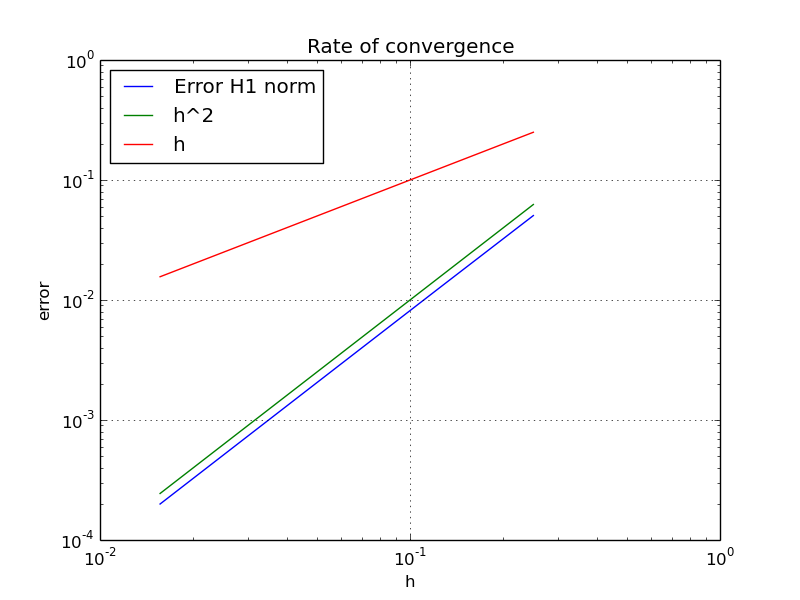
\includegraphics[width=\textwidth]{images/convergence_sine}
\caption{The plot shows a second order convergence, since the blue and green lines are parallel.}
\end{figure}
\vspace{1cm}

\begin{center}
\begin{tabular}{| c | c | c | c | c |}
\hline
$  \mathbf{N}$ & $ \mathbf{|| u_{exact} - u_h ||_{L^2}}$ & $  \mathbf{ | u_{exact} - u_h |_{H^1}}$ & \textbf{Rate in }  $ \mathbf{L^2}$ & \textbf{Rate in } $  \mathbf{H^1}$  \\
\hline
$ 4 $ & $1.9388 \times 10^{-3}$ & $5.0548 \times 10^{-2}$  & & \\
\hline
$ 8$ & $2.4515  \times 10^{-4}$ & $1.2733 \times 10^{-2}$ &  $2.9834$ &  $1.9890$   \\
\hline
$ 16 $ & $ 3.0745 \times 10^{-5}$ & $3.1896 \times 10^{-3}$ & $ 2.9952 $ & $1.9971$   \\
\hline
$ 32$ & $3.8465 \times 10^{-6}$ & $7.9780 \times 10^{-4}$ & $ 2.9987 $ & $ 1.9992 $  \\
\hline
$ 64$ & $4.8092 \times 10^{-7}$ & $1.9948 \times 10^{-4}$  & $ 2.9997 $ & $1.9998$ \\
\hline
\end{tabular}
\end{center}



\begin{center}
\begin{tabular}{| c | c | c |}
\hline
$\mathbf{N}$ & $\mathbf{|| p_{exact} - p_h ||_{L^2}}$ & \textbf{Rate in } $  \mathbf{L^2}$  \\
\hline
$ 4 $ & $1.4420  \times 10^{-4} $ & \\
\hline
$ 8 $ & $ 1.1896  \times 10^{-5} $ & $3.5995$ \\
\hline
$ 16 $ & $ 1.0089  \times 10^{-6} $ & $3.5596$ \\
\hline
$ 32 $ & $  8.7143 \times 10^{-8} $ & $3.5332$ \\
\hline
$ 64 $ & $ 8.0070 \times 10^{-9} $ & $3.4440$ \\
\hline
\end{tabular}
\end{center}




\section{Pressure-driven channel flow (2D)}
% References:
% Fenics book
% http://faculty.kfupm.edu.sa/CHE/usamah/CHE204/CHE204-HD22%20-%20Flow%20Through%20Circular%20Pipe.pdf

% Should I add some theory on this?

A typical test problem is finding the solution of the Navier-Stokes equations in a two-dimensional pressure-driven channel. We consider a viscous flow between parallel plates, where the geometry is the unit square $[0,1]^2$, and the kinematic viscosity is $\nu = 1/8$. We assume that both plates are fixed, i.e. no-slip boundary conditions are applied to the velocity at the upper and lower walls, and Neumann boundary conditions $\sigma \cdot \vec{n} = 0$ are applied at the inlet and outlet. Dirichlet boundary conditions are applied to the pressure at the inlet and outlet, with $p = 1$ at the inlet and $p = 0$ at the outlet. The initial condition for the velocity is $\mathbf{u} = (0,0)$. As a reference value in order to verify the agreement of our solution, we use the $x$-component of the velocity at the point $(x, y) = (1, 0.5)$ at final time $T = 0.5 $. The value reported on the FEniCS book [PUT REFERENCE] is $u_x(1, 0.5, T=0.5) \approx 0.44321183655681595$, while the one obtained in our results is $0.443217320106$.

\begin{figure}[h!]
\centering
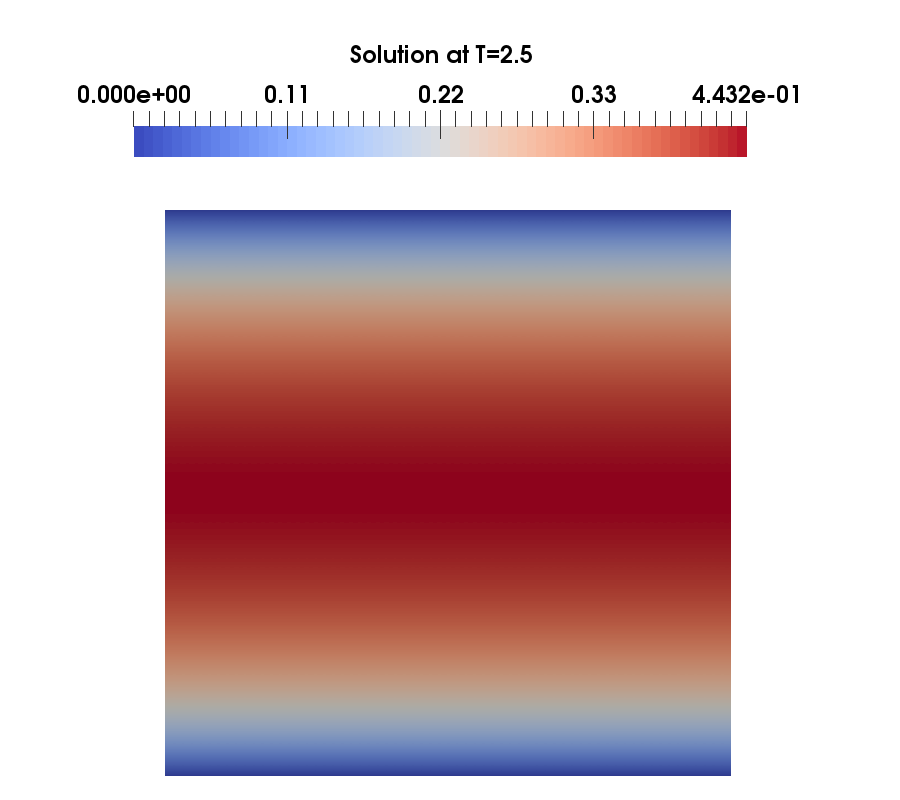
\includegraphics[width=0.8\textwidth]{images/velocity_solution.png}
\caption{The plot shows the solution $u(x,y)$ for $\nu = 1/8$.}
\end{figure}

\begin{figure}[h!]
\centering
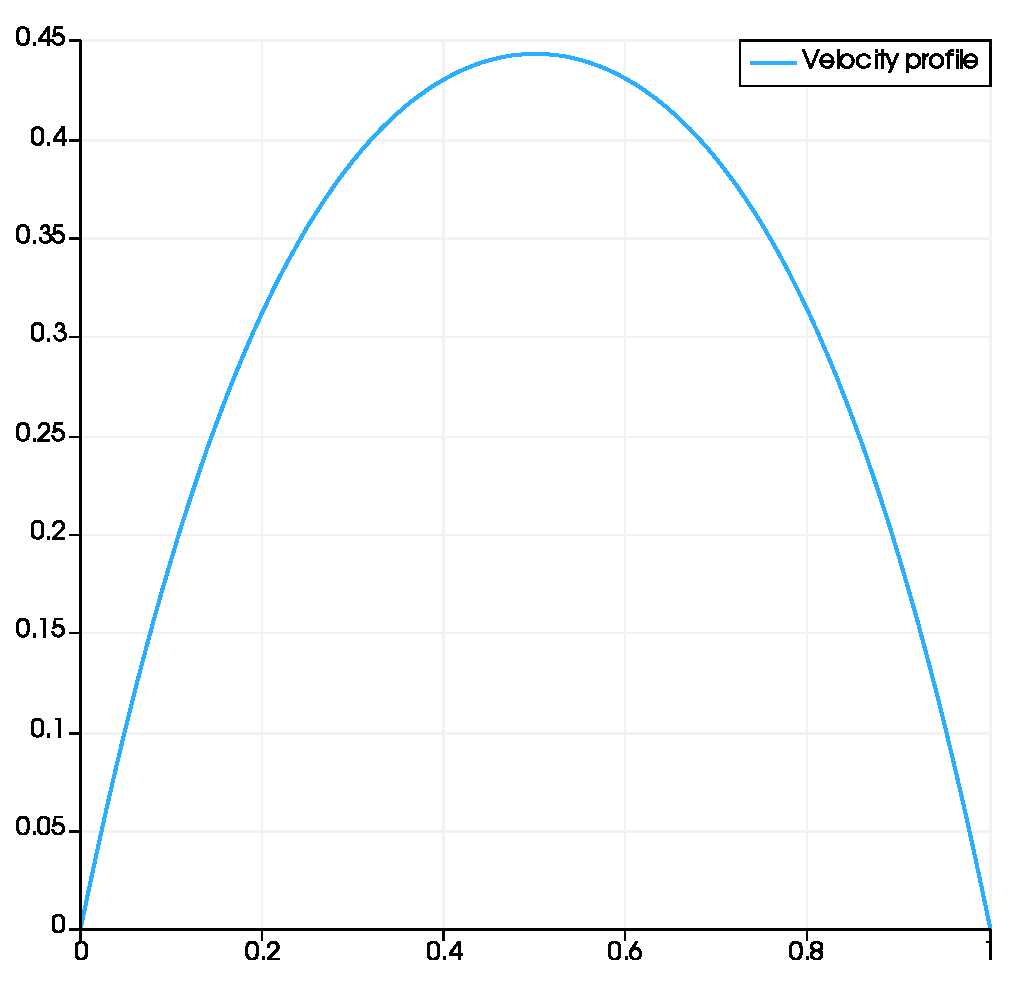
\includegraphics[width=0.6\textwidth]{images/velocity_profile.pdf}
\caption{Velocity profile at the points $(0.5, 1)$ and $(0.5, 0)$.}
\end{figure}

\section{Driven cavity}
% References:
% Fenics book, Quarteroni, Fluid dynamics F. White

A typical benchmark problem for fluid flow solvers in the two-dimensional lid-driven cavity problem. We consider a square cavity $\Omega$ with sides of unit length, i.e. $\Omega = [0,1] \times [0,1]$, kinematic viscosity $\nu = 1/1000$, and density $\rho = 1$. No-slip boundary conditions are imposed on each edge of the square, except at the upper edge where the velocity is set to $\mathbf{u} = (1,0)^T$, as follows

\[
\begin{cases}
\mathbf{u = 0}, & \mbox{on } \partial \Omega \backslash \Gamma \\
\mathbf{u} = (1,0)^T, & \mbox{on } \Gamma
\end{cases}
\]

where $ \Gamma = \set{ \mathbf{x} = (x,y)^T \in \partial \Omega | y = 1}$. We use finite elements on triangular grids of the type $\mathcal{P}_2-\mathcal{P}_1$. The initial condition for the velocity is set to zero. The resulting flow is a vortex developing in the upper right corner and then traveling towards the center of the square as the flow evolves. \\
To verify the correctness of the solver, we consider the minimum of the \textit{stream function}. The stream function $\psi$ allows us to satisfy the continuity equation and then solve the momentum equation directly for the single variable $\psi$. It is defined by

\[
\mathbf{u} = \nabla \times \psi = (\frac{\partial \psi}{\partial y} , - \frac{\partial \psi }{\partial x}),
\]

and it can be computed by solving the Poisson problem

\[
- \nabla^2 \psi = \omega,
\]

where $\omega$ is the vorticity given by

\[
\omega = \nabla \times \mathbf{u} = \frac{\partial u_y}{\partial x} - \frac{\partial u_x}{\partial y}.
\]


As a reference value, we use the one reported on the FEniCS book [REFERENCE], where the solution at the final time $T = 2.5$ was computed using the spectral element code Semtex with up to $80 \times 80$ $10^{th}$ order elements, heavily refined in the area in the vicinity of the minimum of the stream function. The time-stepping for computing the reference solution was handled by a third order implicit discretization, and a very short time step was used to minimize temporal errors.  The obtained reference value was $min(\psi) = -0.061 077$.

\begin{figure}[ht]
\centering
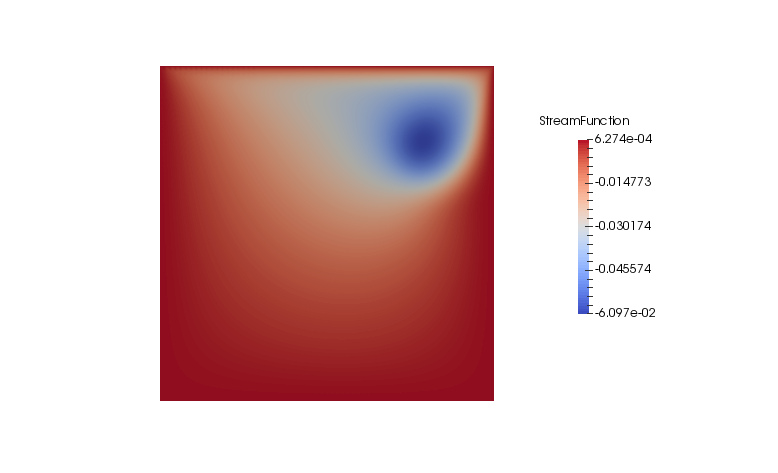
\includegraphics[width=\textwidth]{images/oyvind.png}
\vspace{-1cm}
\caption{The plot shows the stream function, and its minimum value $-0.06097$ (THIS IS OYVIND'S ).}
\end{figure}


In our case, a Crank-Nicolson (second order) discretization was used, with $\theta = 0.5$. A $64 \times 64$ number of elements was used, with $dt = 0.0125$ as time step. Hence, the obtained value was $min(\psi) = -0.061 121$, in fair agreement with the reference one. \\

\vspace{-.3cm}
\begin{figure}[ht]
\centering
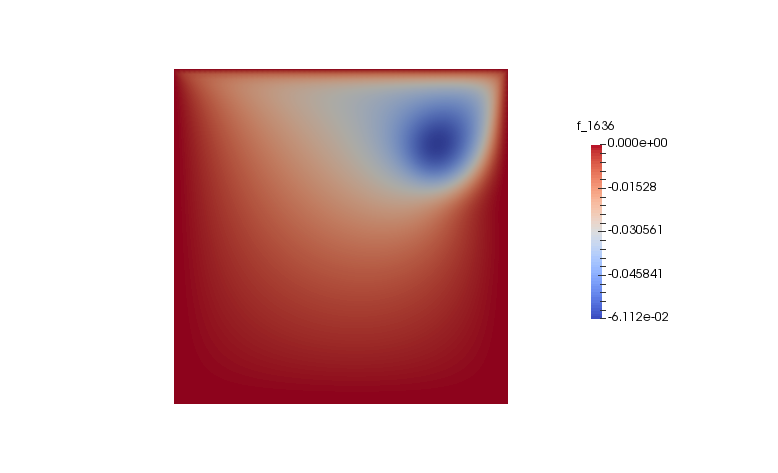
\includegraphics[width=\textwidth]{images/mine.png}
\vspace{-1cm}
\caption{The plot shows the stream function, and its minimum value $-0.061 121$.}
\end{figure}

(MISSING: PUT MY STREAM FUNCTION, OYVIND'S, AND THE ERROR BETWEEN THEM. \\
NOTE: Oyvind's stream function minimum is not exactly the same as the fenics book, what should I put then as a reference?)


\section{ALE test case}
See Vegard
\section{ALE + elasticity test case}

\chapter{Numerical results}

\chapter{Discussion}

\chapter{Conclusions}

\end{document}
